\section{Fairness in bipartite ranking}

\subsection{Motivation}
\begin{frame}{Motivation}
    \begin{itemize}
        \item Most of \gbf{fairness-aware} machine learning research focuses on \gbf{classification} models.
        \item Because bipartite ranking models are evaluated differently (\textit{i.e}, with ROC curves), evaluating fairness for bipartite ranking models might be \gbf{more challenging}.        
        \item However, learning a scoring function over a classifier adds \gbf{more flexibility} to the thresholds, which means that a fair scoring function will lead to \gbf{fair decisions for all thresholds of interest}.
    \end{itemize}
\end{frame}


\subsection{AUC-based constraints}
\begin{frame}{AUC-based constraints}

    \blfootnote{Reminder : $G_s(t) = \mathbf{P}\{s(X) \leq t | Y = +1\}$ and $H_s(t) = \mathbf{P}\{s(X) > t | Y = -1\}$}
    
    Previous works proposed to use \gbf{AUC-based constraints} to ensure fairness in bipartite ranking models. Let's denote $G_s^{(i)}$ (resp. $H_s^{(i)}$) the CDF of the score on the positive (resp. negatives) of group $z \in \{0,1\}$.
    
    \citeauthor{beutel2019fairness}\footcite{beutel2019fairness} proposed to use \gbf{intra-group pairwise} AUC fairness :
    \begin{equation}
        AUC_{H_s^{(0)},G_s^{(0)}} = AUC_{H_s^{(1)},G_s^{(1)}}
    \end{equation}

    

\end{frame}


\begin{frame}{AUC-based constraints}

    \blfootnote{Reminder : $G_s(t) = \mathbf{P}\{s(X) \leq t | Y = +1\}$ and $H_s(t) = \mathbf{P}\{s(X) > t | Y = -1\}$}
    
    \citeauthor{borkan2019nuanced}\footcite{borkan2019nuanced} proposed to use \gbf{Background Negative Subgroup Positive (BNSP)} AUC fairness :

    \begin{equation}
        AUC_{H_s,G_s^{(0)}} = AUC_{H_s,G_s^{(1)}}
    \end{equation}
    
    Finally, \citeauthor{kallus2019fairness}\footcite{kallus2019fairness} proposed to use \gbf{inter-group pairwise} AUC fairness :

    \begin{equation}
        AUC_{H_s^{(0)},G_s^{(1)}} = AUC_{H_s^{(1)},G_s^{(0)}}
    \end{equation}

\end{frame}
    

\begin{frame}{AUC-based constraints}


    {\large\textbf{What is the difference ?}}
    \begin{itemize}
        \item \textbf{Intra-group fairness} : equal performance \gbf{within} groups
        \item \textbf{Background Negative Subgroup Positive fairness} : positives \gbf{from either
        group} have the \gbf{same probability of being ranked higher} than a negative example
        \item \textbf{Inter-group fairness} (in this specific case) : positives of a group can be distinguished from the \gbf{negatives of the other group} as effectively for both groups
    \end{itemize}


\end{frame}


\begin{frame}{AUC-based constraints}
    There are \gbf{many more constraints} available !\footnote{If you're interested, check out the supplementary material of the original paper}. This is one of the \gbf{strengths} of the method proposed by the authors : \gbf{it can be adapted to any fairness constraint} we might be interested in thanks to the following framework :

    \begin{align} \label{eq:auc-based-constraints-general}
        AUC_{\alpha^\top D(s), \beta^\top D(s)} = AUC_{\alpha'^\top D(s),
        \beta'^\top D(s)}.
    \end{align}

    with $ D(s) := (H^{(0)}_s, H^{(1)}_s, G^{(0)}_s, G^{(1)}_s)^\top$ and the probability vectors $\alpha, \beta, \alpha', \beta' \in  \mathcal{P}$ where $\mathcal{P} = \{ v \mid v \in \mathbb{R}_+^4, \mathbf{1}^\top v = 1 \}$.

\end{frame}


\begin{frame}{AUC-based constraints}
    Equation \ref{eq:auc-based-constraints-general} is \gbf{under-specified}, so the authors finally formulate all \gbf{relevant} constraints as a linear combination of \gbf{5 elementary constraints}.

    \vspace{-0.85cm} 
    \begin{align*}
        C_1(s) &= AUC_{H^{(0)}_s, H^{(1)}_s} - 1/2,\\
        C_2(s) &=   1/2 - AUC_{G^{(0)}_s, G^{(1)}_s},\\
        C_3(s) &= AUC_{H^{(0)}_s, G^{(0)}_s} - AUC_{H^{(0)}_s, G^{(1)}_s}, \\
        C_4(s) &= AUC_{H^{(0)}_s, G^{(1)}_s} - AUC_{H^{(1)}_s, G^{(0)}_s}, \\
        C_5(s) &= AUC_{H^{(1)}_s, G^{(0)}_s} - AUC_{H^{(1)}_s, G^{(1)}_s}.
    \end{align*}


    The family of fairness constraints we consider is then the set of linear
    combinations of the $C_l(s) = 0$:
    \begin{align}\label{eq:barycenter-constraint-formulation}
        \mathcal{C}_\Gamma(s): \quad \Gamma^\top C(s) &= \textstyle\sum_{l=1}^5
        \Gamma_l C_l (s) = 0,
    \end{align}

    where $\Gamma = (\Gamma_1 , \dots, \Gamma_5)^\top \in \mathbb{R}^5$.


\end{frame}


\begin{frame}{AUC-based constraints}
    
    The \gbf{learning problem} is defined as : 

    \begin{align*}
        \label{eq:auc_general_problem}
            \max_{s\in\mathcal{S}} \quad AUC_{H_s,G_s} - \lambda |\Gamma^\top C(s)|,
    \end{align*}
    where $\lambda \ge 0$ is a hyperparameter balancing ranking performance and fairness.

    For example, for the \gbf{intra-group pairwise} AUC fairness constraint, we have :

    \begin{align*}
        L_\lambda(s) := AUC_{H_s,G_s} - \lambda \big|AUC_{H^{(0)}_s, G^{(0)}_s} - AUC_{ H^{(1)}_s, G^{(1)}_s }\big|.
    \end{align*}

\end{frame}



\begin{frame}{Limits of AUC-based constraints}
    \begin{figure}[t]
        \centering
        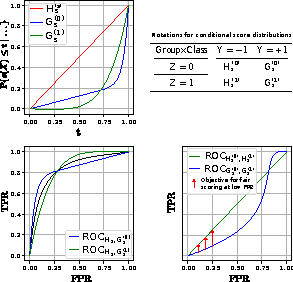
\includegraphics[width=0.6\columnwidth, trim = 0cm 0cm 2.35cm 2.4cm, clip]{images/original_paper/example_simple_dists_explained_with_table2.pdf}
        \caption{Illustrating the limitations of $AUC$-based fairness.}
        \label{fig:example-1}
    \end{figure}
\end{frame}

\subsection{ROC-based constraints}
\begin{frame}{ROC-based constraints}

    For $\alpha \in [0,1]$, consider the deviations between the \gbf{positive} (resp. \gbf{negative}) \gbf{inter-group ROCs} and the \gbf{identity function}:
    \begin{align*}
        \Delta_{G, \alpha}(s) &:= ROC_{G^{(0)}_s, G^{(1)}_s}(\alpha) - \alpha, \\
        \big( \text{resp. } \Delta_{H, \alpha}(s) & := ROC_{H^{(0)}_s,H^{(1)}_s}
        (\alpha) - \alpha
        \big).
    \end{align*}


    Ideally, we would want $\Delta_{G, \alpha}(s)$ and $\Delta_{H, \alpha}(s)$ to be equal to 0 for all $\alpha \in [0,1]$.

    But this will most likely \gbf{jeopardize} the ranking performance as it is \gbf{too restrictive} !
    
\end{frame}

\begin{frame}{ROC-base constraints}

    Instead, the authors propose a general approach to implement the satistifaction of a \gbf{finite number of fairness constraints} denoted by $m_H,m_G \in \mathbf{N}$ for the negatives and the positives respectively. We define $\alpha_{H} = [\alpha_H^{(1)},\dots,\alpha_H^{(m_H)}]\in[0,1]^{m_H}$ and $\alpha_{G} = [\alpha_G^{(1)},\dots,\alpha_G^{(m_G)}]\in[0,1]^{m_G}$ the points at which they apply (sorted in strictly increasing order).

    The \gbf{learning objective} becomes:
    \begin{align*}
        L_\Lambda(s) = 
        AUC_{H_s,G_s} &- 
        \sum_{k=1}^{m_H} \lambda_H^{(k)}  \big| \Delta_{H,\alpha_H^{
        (k)}}(s) \big| 
        - \sum_{k=1}^{m_G} \lambda_G^{(k)} \big| \Delta_{G,\alpha_G^{(k)}}(s) \big|,
    \end{align*}
     
    $\lambda_H=[\lambda_H^{(1)},\dots,\lambda_H^{(m_H)}]\in \mathbf{R}_+^
    {m_H}$ and $\lambda_G=[\lambda_G^{(1)},\dots,\lambda_G^{(m_G)}]\in \mathbf{R}_+^{m_G}$ are
    hyperparameters.
    
\end{frame}